\documentclass{beamer}
\mode<presentation> {
%\usetheme{Madrid}
%\usetheme{default}
\usepackage{color}
\definecolor{bottomcolour}{rgb}{0.21,0.11,0.21}
\definecolor{middlecolour}{rgb}{0.21,0.11,0.21}
\setbeamercolor{structure}{fg=white}
\setbeamertemplate{frametitle}[default]%[center]
\setbeamercolor{normal text}{bg=black, fg=white}
\setbeamertemplate{background canvas}[vertical shading]
[bottom=bottomcolour, middle=middlecolour, top=black]
\setbeamertemplate{items}[circle]
\setbeamertemplate{navigation symbols}{} %no nav symbols
\setbeamercolor{block title}{use=structure,fg=white,bg=structure.fg!50!red!50!blue!100!green}
\setbeamercolor{block body}{parent=normal text,use=block title,bg=block title.bg!5!white!10!bg,fg=white}
\setbeamertemplate{navigation symbols}{}
}

\usepackage{graphicx} 
\usepackage{booktabs} 
\usepackage[utf8]{inputenc}  
\usepackage[T1]{fontenc}  
\usepackage{geometry}     
\usepackage[francais]{babel} 
\usepackage{eurosym}
\usepackage{verbatim}
\usepackage{ragged2e}
\justifying

%%%%%%%%%%%%%%%%%%%%%%%%%%%%%%%%%%%%%%%%%%%%%%%%%%%%%%%%%%%%%%%%
%% ccBeamer 0.1, 2007-07-02                                   %%
%% Written by Sebastian Pipping <webmaster@hartwork.org>      %%
%% ---------------------------------------------------------- %%
%% Licensed under Creative Commons Attribution-ShareAlike 3.0 %%
%% http://creativecommons.org/licenses/by-sa/3.0/             %%
%%%%%%%%%%%%%%%%%%%%%%%%%%%%%%%%%%%%%%%%%%%%%%%%%%%%%%%%%%%%%%%%


%% Images
\newcommand{\CcImageBy}[1]{%
	
\includegraphics[scale=#1]{creative_commons/cc_by_30.pdf}%
}
\newcommand{\CcImageCc}[1]{%
	
\includegraphics[scale=#1]{creative_commons/cc_cc_30.pdf}%
}
\newcommand{\CcImageDevNations}[1]{%
	
\includegraphics[scale=#1]{creative_commons/cc_dev_nations_30.pdf}%
}
\newcommand{\CcImageNc}[1]{%
	
\includegraphics[scale=#1]{creative_commons/cc_nc_30.pdf}%
}
\newcommand{\CcImageNd}[1]{%
	
\includegraphics[scale=#1]{creative_commons/cc_nd_30.pdf}%
}
\newcommand{\CcImagePd}[1]{%
	
\includegraphics[scale=#1]{creative_commons/cc_pd_30.pdf}%
}
\newcommand{\CcImageSa}[1]{%
	
\includegraphics[scale=#1]{creative_commons/cc_sa_30.pdf}%
}
\newcommand{\CcImageSampling}[1]{%
	
\includegraphics[scale=#1]{creative_commons/cc_sampling_30.pdf}%
}
\newcommand{\CcImageSamplingPlus}[1]{%
	
\includegraphics[scale=#1]{creative_commons/cc_sampling_plus_30.pdf}%
}


%% Groups
\newcommand{\CcGroupBy}[1]{% zoom
	\CcImageBy{#1}%
}
\newcommand{\CcGroupByNc}[2]{% zoom, gap
	\CcImageBy{#1}\hspace*{#2}\CcImageNc{#1}%
}
\newcommand{\CcGroupByNcNd}[2]{% zoom, gap
	\CcImageBy{#1}\hspace*{#2}\CcImageNc{#1}\hspace*{#2}\CcImageNd{#1}%
}
\newcommand{\CcGroupByNcSa}[2]{% zoom, gap
	\CcImageBy{#1}\hspace*{#2}\CcImageNc{#1}\hspace*{#2}\CcImageSa{#1}%
}
\newcommand{\CcGroupByNd}[2]{% zoom, gap
	\CcImageBy{#1}\hspace*{#2}\CcImageNd{#1}%
}
\newcommand{\CcGroupBySa}[2]{% zoom, gap
	\CcImageBy{#1}\hspace*{#2}\CcImageSa{#1}%
}
\newcommand{\CcGroupDevNations}[1]{% zoom
	\CcImageDevNations{#1}%
}
\newcommand{\CcGroupNcSampling}[2]{% zoom, gap
	\CcImageNc{#1}\hspace*{#2}\CcImageSampling{#1}%
}
\newcommand{\CcGroupPd}[1]{% zoom
	\CcImagePd{#1}%
}
\newcommand{\CcGroupSampling}[1]{% zoom
	\CcImageSampling{#1}%
}
\newcommand{\CcGroupSamplingPlus}[1]{% zoom
	\CcImageSamplingPlus{#1}%
}


%% Text
\newcommand{\CcLongnameBy}{Attribution}
\newcommand{\CcLongnameByNc}{Attribution-NonCommercial}
\newcommand{\CcLongnameByNcNd}{Attribution-NoDerivs}
\newcommand{\CcLongnameByNcSa}{Attribution-NonCommercial-ShareAlike}
\newcommand{\CcLongnameByNd}{Attribution-NoDerivs}
\newcommand{\CcLongnameBySa}{Attribution-ShareAlike}

\newcommand{\CcNote}[1]{% longname
	This work is licensed under the \textit{Creative Commons #1 3.0 License}.%
}


\title[Les métadonnées]{Les métadonnées} 
\author{Genma}

\begin{document}

%% Titlepage
\begin{frame}
	\titlepage
	\vfill
	\begin{center}
		\CcGroupByNcSa{0.83}{0.95ex}\\[2.5ex]
		{\tiny\CcNote{\CcLongnameByNcSa}}
		\vspace*{-2.5ex}
	\end{center}
\end{frame}

%----------------------------------------------------------------------------------------
\begin{frame}
\Huge{\centerline{Les métadonnées}}
\end{frame}

\begin{frame}
\frametitle{Les métadonnées}
\begin{block}{Qu'est-ce qu'une metadonnée ?}
\justifying{
Une métadonnée est une information qui caractérise une donnée. 
\\~\\
Prenons un exemple : lorsque vous créez un PDF, en général, des données additionnelles sont ajoutées à votre fichier : le nom du logiciel producteur, votre nom, la date de production, la description de votre document, le titre de votre document, la dernière date de modification, … ce sont des métadonnées. 
\\~\\
Vous n'avez peut-être pas envie de partager ces informations lorsque vous partagez votre fichier.}
\end{block}
\end{frame}


%------------------------------------------------

\begin{frame}
\frametitle{Metadata}
\begin{center}
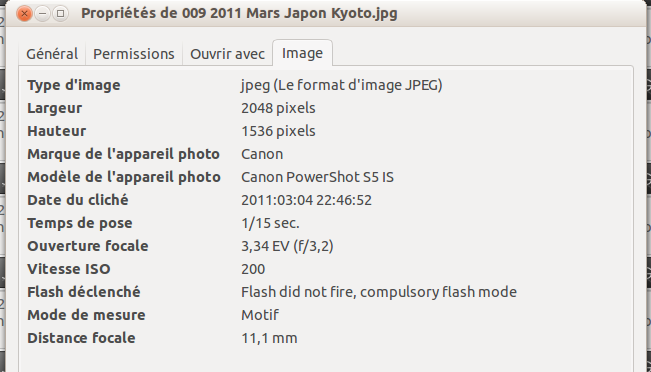
\includegraphics[scale=0.5] {./materials/Metadata.png} 
\end{center}
\end{frame}


\begin{frame}
\frametitle{Les métadonnées}
\begin{block}{Pourquoi les métadonnées sont elles un risque pour notre vie privée?}
\justifying{
Les métadonnées dans un fichier peuvent en dire beaucoup sur vous. Les appareils photos enregistrent des données sur le moment où une photo a été prise et quel appareil photo a été utilisé. 
\\~\\
Les documents bureautiques ajoutent automatiquement l'auteur et diverses informations sur la société aux documents et feuilles de calcul. 
\\~\\
Peut-être que vous ne voulez pas divulguer ces informations sur le web?
}
\end{block}
\end{frame}

%------------------------------------------------

\begin{frame}
\frametitle{Le logiciel MAT}
\begin{block}{Le logiciel MAT}
\justifying{
MAT est une boîte à outil composé d'une interface graphique, d'une version en ligne de commande et d'une bibliothèque.
\\~\\
MAT crée automatiquement une copie des documents originaux dans une version nettoyée (laissant intact les originaux). 
\\~\\
MAT est fournit par défaut dans le live-cd Tails. 
}
\end{block}
\end{frame}

%------------------------------------------------

\begin{frame}
\frametitle{Le logiciel MAT}
\begin{center}
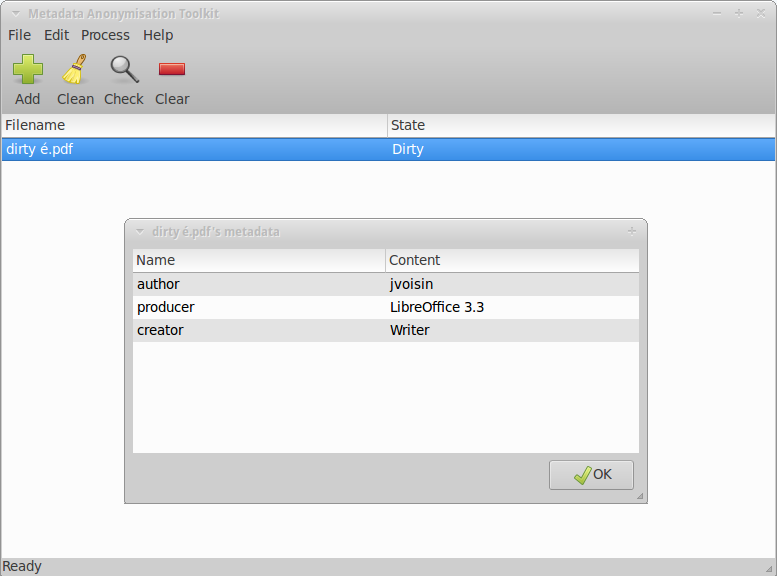
\includegraphics[scale=0.3] {./materials/Mat.png} 
\end{center}
\end{frame}


%------------------------------------------------
\begin{frame}
\frametitle{MAT}

\begin{block}{Les formats actuellement supportés}
Actuellement, MAT supporte pleinement les formats suivants :
\begin{itemize}
\item Portable Network Graphics (.png)
\item JPEG (.jpg, .jpeg, …)
\item Open Documents (.odt, .odx, .ods, …)
\item Office OpenXml (.docx, .pptx, .xlsx, …)
\item Portable Document Fileformat (.pdf)
\item Tape ARchives (.tar, .tar.bz2, …)
\item MPEG AUdio (.mp3, .mp2, .mp1, …)
\item Ogg Vorbis (.ogg, …)
\item Free Lossless Audio Codec (.flac)
\item Torrent (.torrent)
\end{itemize}
\end{block}
\end{frame}

%------------------------------------------------

\begin{frame}
\frametitle{Le logiciel MAT}
\begin{block}{Pourquoi MAT n'est pas la solution ultime?}
\justifying{
MAT ne fait que supprimer les metadonnées de vos fichiers, il n'anonymise pas leur contenu, ni ne gère les filigranes, la stéganographie, ou tout autre personnalisation excessive des métadonnées. 
\\~\\
Si vous voulez réellement être anonyme, utilisez un format qui ne contient pas de métadonnées, ou mieux : utilisez du texte brut.
\\~\\
Et encore plus important, faites attention : chaque format peut-être "watermarked" / avoir un tatouage-marquage numérique.
}
\end{block}
\end{frame}

%------------------------------------------------

\begin{frame}
\frametitle{Les autres logiciels}

\begin{block}{D'autres outils du même type}
\begin{itemize}
\item Exiftool : \url{http://www.sno.phy.queensu.ca/~phil/exiftool/}
\item exiv2 : \url{http://www.exiv2.org/}
\item jhead : \url{http://www.sentex.net/~mwandel/jhead/}
\item Metanull
\end{itemize}
\end{block}
\end{frame}

%----------------------------------------------------------------------------------------
\begin{frame}
\Huge{\centerline{Merci de votre attention.}}
\Huge{\centerline{Place aux questions. Débattons...}}
\end{frame}

\end{document}
